\documentclass[aspectratio=169, table]{beamer}

\usepackage{listings}
\usepackage{tikz}
\usetikzlibrary{arrows.meta, positioning}


\lstdefinestyle{RustStyle}{
	language=Java,
	morekeywords={println, Ok, async, fn, main, use, let, mut},
	basicstyle=\ttfamily\scriptsize,
	keywordstyle=\color{blue},
	commentstyle=\color{gray},
	stringstyle=\color{red},
	breaklines=true,
	showstringspaces=false,
	tabsize=2,
	captionpos=b,
	numbers=left,
	numberstyle=\tiny\color{gray},
	frame=lines,
	backgroundcolor=\color{lightgray!10},
	comment=[l]{//},
	morecomment=[s]{/*}{*/},
	commentstyle=\color{gray}\ttfamily,
	string=[s]{'}{'},
	morestring=[s]{"}{"},
	stringstyle=\color{teal}\ttfamily,
	%	showstringspaces=false
	literate=
	{\{}{{\textcolor{red}{\{}}}1
	{\}}{{\textcolor{red}{\}}}}1
	{:}{{\textcolor{red}{:}}}1
	{=}{{\textcolor{red}{=}}}1
	{.}{{\textcolor{red}{.}}}1
	{]}{{\textcolor{red}{]}}}1
	{[}{{\textcolor{red}{[}}}1
	{\#}{{\textcolor{red}{\#}}}1
	{;}{{\textcolor{red}{;}}}1
	{?}{{\textcolor{red}{?}}}1
	{!}{{\textcolor{red}{!}}}1
}

%\usepackage[beamertheme=./praditatheme]{Pradita}

\usetheme{Pradita}

\lstdefinelanguage{bash} {
	keywords={},
	basicstyle=\ttfamily\small,
	keywordstyle=\color{blue}\bfseries,
	ndkeywords={iex},
	ndkeywordstyle=\color{purple}\bfseries,
	sensitive=true,
	commentstyle=\color{gray},
	stringstyle=\color{red},
	numbers=left,
	numberstyle=\tiny\color{gray},
	breaklines=true,
	frame=lines,
	backgroundcolor=\color{lightgray!10},
	tabsize=2,
	comment=[l]{\#},
	morecomment=[s]{/*}{*/},
	commentstyle=\color{gray}\ttfamily,
	stringstyle=\color{purple}\ttfamily,
	showstringspaces=false
}

\lstdefinestyle{JavaStyle}{
	language=Java,
	basicstyle=\ttfamily\footnotesize,
	morekeywords={String, int},
	keywordstyle=\color{blue},
	commentstyle=\color{gray},
	stringstyle=\color{red},
	breaklines=true,
	showstringspaces=false,
	tabsize=2,
	captionpos=b,
	numbers=left,
	numberstyle=\tiny\color{gray},
	frame=lines,
	backgroundcolor=\color{lightgray!10},
	comment=[l]{//},
	morecomment=[s]{/*}{*/},
	commentstyle=\color{gray}\ttfamily,
	string=[s]{'}{'},
	morestring=[s]{"}{"},
	%	stringstyle=\color{teal}\ttfamily,
	%	showstringspaces=false
}

\title{\LARGE Pipeline/Pipe-and-Filter\\Architecture\\\vspace{10pt}}
\subtitle{IF231303-Software Architecture}
\author{\textbf{Alfa Yohannis}}
\begin{document}
	
	\frame{\titlepage}
	

	\begin{frame}[fragile]
		\frametitle{Contents}
		\vspace{20pt}
		\begin{columns}[t]
			\column{0.5\textwidth}
			\tableofcontents[sections={1-4}]
			
			\column{0.5\textwidth}
			\tableofcontents[sections={5-10}]
		\end{columns}
	\end{frame}

\section{Example Diagram}
	\begin{frame}{Diagram: Pipe-and-Filter Architecture}
	\centering
	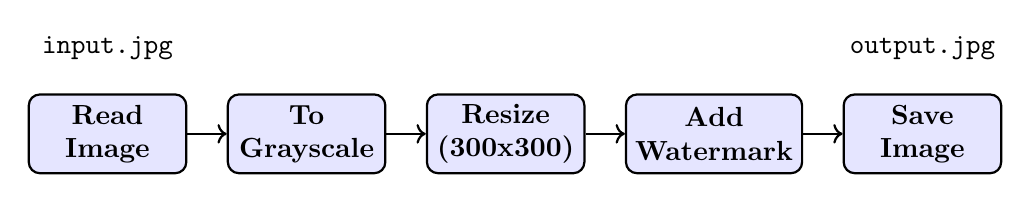
\begin{tikzpicture}[
		node distance=1.6cm and .5cm,
		box/.style={draw, thick, rounded corners, minimum width=2cm, minimum height=1cm, align=center, fill=blue!10},
		arrow/.style={->, thick}
		]
		
		% Nodes
		\node[box] (read) {\textbf{Read}\\\textbf{Image}};
		\node[box, right=of read] (gray) {\textbf{To}\\\textbf{Grayscale}};
		\node[box, right=of gray] (resize) {\textbf{Resize}\\\textbf{(300x300)}};
		\node[box, right=of resize] (watermark) {\textbf{\textbf{Add}}\\\textbf{Watermark}};
		\node[box, right=of watermark] (save) {\textbf{Save}\\\textbf{Image}};
		
		% Arrows
		\draw[arrow] (read) -- (gray);
		\draw[arrow] (gray) -- (resize);
		\draw[arrow] (resize) -- (watermark);
		\draw[arrow] (watermark) -- (save);
		
		% Optional labels
		\node[above=0.3cm of read] {\texttt{\textbf{input.jpg}}};
		\node[above=0.3cm of save] {\texttt{\textbf{output.jpg}}};
		
	\end{tikzpicture}
\end{frame}

\section{Introduction}

\begin{frame}[fragile]{Introduction to Pipe-and-Filter Architecture}
	\vspace{20pt}
	\begin{columns}[T]
		\column{0.5\textwidth}
		Modern systems demand architectures that are:
		\begin{itemize}
			\item Modular
			\item Maintainable
			\item Efficient in data handling
		\end{itemize}
		
		\textbf{Pipe-and-Filter Architecture} addresses these needs by dividing tasks into independent \textit{filters} connected via \textit{pipes}.
		
		Common use cases:
		\begin{itemize}
			\item Compilers
			\item Multimedia processing
			\item Big data pipelines
		\end{itemize}
		
		\column{0.5\textwidth}
		\textbf{Key strengths:}
		\begin{itemize}
			\item Flexible system design
			\item Supports parallel and streaming processing
		\end{itemize}
		
		This chapter explains:
		\begin{itemize}
			\item Core concepts and components
			\item Benefits and limitations
			\item Practical examples and use cases
		\end{itemize}
		
		Focus: clear understanding without diving deep into advanced optimisations.
	\end{columns}
\end{frame}


\section{Examples of Application}

\begin{frame}[fragile]{Applications of Pipe-and-Filter Architecture}
	\vspace{20pt}
	\begin{columns}[T]
		\column{0.5\textwidth}
		\textbf{Text Processing:}
		\begin{itemize}
			\item Classic use: \textbf{Compiler pipeline}
			\item Stages: lexical analysis, parsing, semantic check, code generation
			\item Also used in email filtering, log analysis, and info extraction
		\end{itemize}
		
		\textbf{Multimedia:}
		\begin{itemize}
			\item Video: decode $\rightarrow$ scale $\rightarrow$ render
			\item Audio: filter noise $\rightarrow$ normalize $\rightarrow$ compress
		\end{itemize}
		
		\column{0.5\textwidth}
		\textbf{Big Data and Streaming:}
		\begin{itemize}
			\item ETL: extract $\rightarrow$ transform $\rightarrow$ load
			\item Streaming: Kafka, Flink
			\item Filters run in parallel for scalability
		\end{itemize}
		
		\textbf{Why it works:}
		\begin{itemize}
			\item Modular stages
			\item Easy to scale and maintain
			\item Suitable for real-time data flow
		\end{itemize}
	\end{columns}
\end{frame}

\section{Strengths and Limitations}

\begin{frame}[fragile]{Pros and Cons of Pipe-and-Filter Architecture}
	\vspace{20pt}
	\begin{columns}[T]
		\column{0.5\textwidth}
		\textbf{Advantages:}
		\begin{itemize}
			\item \textbf{Modular:} Each filter does one task, making development, testing, and maintenance easier
			\item \textbf{Reusable:} Filters can be reused across different pipelines with minimal changes
			\item \textbf{Parallel:} Filters work independently and can run in parallel for better performance
		\end{itemize}
		
		\column{0.5\textwidth}
		\textbf{Disadvantages:}
		\begin{itemize}
			\item \textbf{Communication Overhead:} Data must flow through pipes, which can add latency or cost
			\item \textbf{Not for Complex Interaction:} Harder to implement feedback loops or two-way communication between filters
			\item \textbf{Linear Flow Constraint:} Less suitable for dynamic or tightly coupled component interactions
		\end{itemize}
	\end{columns}
\end{frame}

\section{Core Concepts}

\begin{frame}[fragile]{Pipe-and-Filter: Key Concepts}
	\vspace{20pt}
	\begin{columns}[T]
		\column{0.5\textwidth}
		\textbf{Filter and Pipe:}
		\begin{itemize}
			\item \textbf{Filter:} Independent unit that transforms input to output
			\item \textbf{Pipe:} Connects filters and transfers data in sequence
			\item Output of one filter feeds directly into the next
		\end{itemize}
		
		\textbf{Sequential Flow:}
		\begin{itemize}
			\item One-way data flow, like an assembly line
			\item Filters work independently with no shared context
		\end{itemize}
		
		\column{0.5\textwidth}
		\textbf{Characteristics:}
		\begin{itemize}
			\item \textbf{Stateless:} Easier to test and debug
			\item \textbf{Streaming-friendly:} Process data on the fly
			\item \textbf{Structured:} Clear and traceable flow
		\end{itemize}
		
		\textbf{Benefit:}
		\begin{itemize}
			\item Simplifies complex systems into modular steps
		\end{itemize}
	\end{columns}
\end{frame}

\section{Main Components}

\begin{frame}[fragile]{Core Components of Pipe-and-Filter}
	\vspace{20pt}
	\begin{columns}[T]
		\column{0.5\textwidth}
		\textbf{Filter:}
		\begin{itemize}
			\item Processes data (e.g., transform, validate, extract)
			\item Each filter has one clear responsibility
			\item Modular, testable, and reusable
			\item Examples: parsing, normalisation, decoding
		\end{itemize}
		
		\textbf{Pipe:}
		\begin{itemize}
			\item Transfers data between filters
			\item Can be memory, file, or network-based
			\item Transparent, no processing logic
		\end{itemize}
		
		\column{0.5\textwidth}
		\textbf{Driver / Controller (Optional):}
		\begin{itemize}
			\item Manages filter execution and data flow
			\item Handles errors or scheduling if needed
			\item Doesn’t alter data directly
		\end{itemize}
		
		\textbf{Summary:}
		\begin{itemize}
			\item Filters do the work
			\item Pipes connect them
			\item Controllers coordinate (if required)
		\end{itemize}
	\end{columns}
\end{frame}

\section{Workflow and Processing Model}

\begin{frame}[fragile]{Pipe-and-Filter: Processing Model}
	\vspace{20pt}
	\begin{columns}[T]
		\column{0.5\textwidth}
		\textbf{Linear Flow:}
		\begin{itemize}
			\item Data flows step-by-step
			\item Simple, predictable logic
			\item \textbf{Example:} Compiler stages – lexical, parsing, semantic, code gen
		\end{itemize}
		
		\textbf{Topology Variants:}
		\begin{itemize}
			\item \textbf{Branching:} Split flow by condition
			\item \textbf{Merging:} Combine multiple flows
			\item \textbf{Example:} Email – spam detection and topic classification
		\end{itemize}
		
		\column{0.5\textwidth}
		\textbf{Parallel Processing:}
		\begin{itemize}
			\item Filters run independently
			\item Improves performance and throughput
			\item \textbf{Example:} IoT – parallel sensor streams (temp, humidity)
			\item \textbf{Example:} Image service – resize, watermark, convert in parallel
		\end{itemize}
		
		\textbf{Key Point:}
		\begin{itemize}
			\item Flexible flow: linear, branched, or parallel
		\end{itemize}
	\end{columns}
\end{frame}

\section{Simple Implementation}

\begin{frame}[fragile]{Simple Pipe-and-Filter Implementation}
	\vspace{20pt}
	\begin{columns}[T]
		\column{0.5\textwidth}
		\textbf{Case Overview:}
		\begin{itemize}
			\item Built in Rust for image processing
			\item Input from \texttt{input/} folder, output to \texttt{output/}
			\item Steps: grayscale, resize, watermark, save as JPEG
			\item Each step = a separate, reusable filter
		\end{itemize}
		
		\textbf{Goal:}
		\begin{itemize}
			\item Modular design for easy testing and maintenance
			\item Clear transformation pipeline for each image
		\end{itemize}
		
		\column{0.5\textwidth}
		\textbf{Pipeline Design:}
		\begin{itemize}
			\item \texttt{read\_image}: load image from file
			\item \texttt{to\_grayscale}: convert to grayscale
			\item \texttt{resize}: scale to 300x300 pixels
			\item \texttt{add\_watermark}: embed text using a font file
			\item \texttt{save\_image}: export as JPEG
		\end{itemize}
		
		\textbf{Note:}
		\begin{itemize}
			\item Filters are connected via return values
			\item No explicit pipe objects, but data flow acts as conceptual pipes
		\end{itemize}
	\end{columns}
\end{frame}



%--------------------------------------------

\begin{frame}[fragile]{Rust Code: Image Pipeline (1/3)}
\vspace{10pt}
\begin{lstlisting}[style=RustStyle]
	use ab_glyph::{FontArc, PxScale};
	use image::ImageReader;
	use image::{DynamicImage, Rgba, RgbaImage};
	use imageproc::drawing::draw_text_mut;
	use std::fs;
	
	fn read_image(path: &str) -> DynamicImage {
		ImageReader::open(path).unwrap().decode().unwrap()
	}
	
	fn to_grayscale(img: DynamicImage) -> DynamicImage {
		img.grayscale()
	}
\end{lstlisting}
\end{frame}

\begin{frame}[fragile]{Rust Code: Image Pipeline (2/3)}
\vspace{10pt}
\begin{lstlisting}[style=RustStyle]
	fn resize(img: DynamicImage, width: u32, height: u32) -> DynamicImage {
		img.resize_exact(width, height, image::imageops::FilterType::Lanczos3)
	}
	
	fn add_watermark(img: &DynamicImage, text: &str, font_path: &str) -> RgbaImage {
		let mut img = img.to_rgba8();
		let font_data = fs::read(font_path).expect("Font file not found");
		let font = FontArc::try_from_vec(font_data).expect("Invalid font format");
		let scale = PxScale::from(20.0);
		
		draw_text_mut(&mut img, Rgba([255, 0, 0, 255]), 10, 10, scale, &font, text);
		img
	}
\end{lstlisting}
\end{frame}

\begin{frame}[fragile]{Rust Code: Image Pipeline (3/3)}
\vspace{10pt}
\begin{lstlisting}[style=RustStyle]
	fn save_image(img: &RgbaImage, output_path: &str) {
		let rgb_image = image::DynamicImage::ImageRgba8(img.clone()).into_rgb8();
		rgb_image.save(output_path).unwrap();
	}
	
	fn main() {
		let input_path = "input/input.jpg";
		let output_path = "output.jpg";
		let font_path = "assets/TitilliumWeb-Regular.ttf";
		
		let img = read_image(input_path);
		let img = to_grayscale(img);
		let img = resize(img, 300, 300);
		let img = add_watermark(&img, "Pipe-and-Filter", font_path);
		save_image(&img, output_path);
		
		println!("Gambar berhasil diproses dan disimpan ke {}", output_path);
	}
\end{lstlisting}
\end{frame}



\subsection{Rust Implementation Explanation}

\begin{frame}[fragile]{Rust Pipeline: Filter Overview}
	\vspace{20pt}
	\begin{columns}[T]
		\column{0.5\textwidth}
		\textbf{Overview:}
		\begin{itemize}
			\item Each step = separate function (filter)
			\item Return values = data flow (conceptual pipes)
			\item Linear process from input to output
		\end{itemize}
		
		\textbf{Dependencies:}
		\begin{itemize}
			\item \texttt{image}, \texttt{imageproc}, \texttt{ab\_glyph}, \texttt{std::fs}
		\end{itemize}
		
		\textbf{Functions:} \\
		\textbf{\texttt{read\_image}:}
		\begin{itemize}
			\item Loads file into \texttt{DynamicImage}
		\end{itemize}
		
	
		
		\column{0.5\textwidth}
		
		\textbf{\texttt{to\_grayscale}:}
		\begin{itemize}
			\item Converts image to grayscale
		\end{itemize}
	
		\textbf{\texttt{resize}:}
		\begin{itemize}
			\item Scales image to 300x300 using \texttt{Lanczos3}
		\end{itemize}
		
		\textbf{\texttt{add\_watermark}:}
		\begin{itemize}
			\item Adds red text at (10,10)
			\item Loads font via \texttt{fs::read}
		\end{itemize}
		
		\textbf{\texttt{save\_image}:}
		\begin{itemize}
			\item Converts to RGB and saves as JPEG
		\end{itemize}
	\end{columns}
\end{frame}


\begin{frame}[fragile]{Execution Flow and Characteristics}
	\vspace{20pt}
	\begin{columns}[T]
		\column{0.5\textwidth}
		\textbf{\texttt{main} function:}
		\begin{enumerate}
			\item Read image from \texttt{input/input.jpg}
			\item Convert to grayscale
			\item Resize to 300x300
			\item Add watermark \texttt{"Pipe-and-Filter"}
			\item Save to \texttt{output.jpg}
		\end{enumerate}
		
		\textbf{Outcome:}
		\begin{itemize}
			\item Notifies on success
		\end{itemize}
		
		\column{0.5\textwidth}
		\textbf{Architectural Traits:}
		\begin{itemize}
			\item Filters are modular and reusable
			\item No shared state between stages
			\item Conceptual pipes = return values
		\end{itemize}
		
		\textbf{Why It Works:}
		\begin{itemize}
			\item Suitable for step-by-step tasks
			\item Easily adapted to text or streaming pipelines
			\item Simple, clear, and scalable
		\end{itemize}
	\end{columns}
\end{frame}


\section{Conclusion}

\begin{frame}[fragile]{Conclusion: Pipe-and-Filter Architecture}
	\vspace{20pt}
	\begin{columns}[T]
		\column{0.5\textwidth}
		\textbf{Key Strengths:}
		\begin{itemize}
			\item Modular and maintainable structure
			\item Each filter handles one processing step
			\item Easy to scale and parallelise
			\item Ideal for linear workflows (e.g., compiler, media, big data)
		\end{itemize}
		
		\textbf{Design Benefit:}
		\begin{itemize}
			\item Encourages separation of concerns
			\item Clear and predictable data flow
		\end{itemize}
		
		\column{0.5\textwidth}
		\textbf{Limitations:}
		\begin{itemize}
			\item Less suited for complex, bidirectional interactions
			\item Rigid linear flow may limit flexibility
		\end{itemize}
		
		\textbf{Final Note:}
		\begin{itemize}
			\item Choose based on domain and communication needs
			\item With proper design, it offers an elegant solution for staged processing
		\end{itemize}
	\end{columns}
\end{frame}


\end{document}
